\label{ride-sharing}
\subsubsection{Purpose}

Every subscribed passenger shall be able to activate the ride sharing function in the mobile app or in the web interface. When this mode is enabled, the passenger also has to provide the system with a destination for the ride.

The system, before allocating a taxi, inserts the pending ride in the set of shared rides and tries to identify possible sharing solutions.
With an adequate algorithm it can propose every feasible sharing solution to the passenger, also considering the number of seats available.

The first passenger who reserves a taxi is called the ``owner'' of the ride.
The passenger can choose to join one of the pending rides or to refuse the proposal, becoming the owner of a new ride.

In the first case the system informs the owner of the ride. The new passenger and eventually his crowd, i.e. the travellers, have to go to the meeting point with the owner of the ride in time. If they are not able to do so, the taxi does not wait for them.

In the second case the system allocates the taxi (\autoref{taxi-availability}) and applies the standard procedure (\autoref{standard-call}).  The passenger becomes the owner of the ride.
If there is another passenger willing to share the same ride, the system allows it and redirects this last user to the meeting point with the owner, who is informed as well as the taxi driver.

The system splits the taxi fee among all the passenger proportionally with the distance travelled.

\subsubsection{Scenario 1}
Batman needs a taxi and decides to enable the sharing mode on his cell phone. Batman enters the destination of his travel and the number of seats (one), and calls a taxi.

When Batman submits the form, the system matches the path of Batman's ride with every pending ride started from Batman's area. It finds only one compatible ride and sends it to Batman.

Batman finds that it is Joker's pending ride and refuses to share the ride.
So, the system allocates a new taxi for Batman.

A new user, Robin, is in Batman's area and needs a taxi. He decides to enable the sharing function and the system proposes to him Batman's and Joker's rides.
He chooses Batman's: the system, which has already communicated the location and the time of the start of the ride to Robin, notifies Batman and the taxi driver that there is an additional passenger.

When the taxi arrives, the taxi driver confirms from his mobile app how many passengers he has picked up.

\subsubsection{Use case}
The use case for a ride sharing is shown in~\autoref{usecase-ridesharing}.

\begin{table}
\begin{center}
\begin{tabular}{| l | p{0.6\textwidth} |}
\hline
Actor & Taxi driver and Multiple Passengers \\
\hline
Goal & Goal~\ref{g-share}
\\
\hline
Input condition & The user enables the sharing option from his mobile phone or from the web interface.  \\
\hline
Event Flow &
\begin{enumerate}
	\item The passenger enables the sharing option.
	\item The passenger enters a destination, and the number of required seats.
	\item The system computes the feasible shared rides and proposes them to the passenger.
	\item The passenger can accept one of the sharing options or refuse all of them.
	\item If the passenger refuses, the system executes the standard taxi call \ref{standard-call}, otherwise it notifies the owner of the ride and the taxi driver.
<<<<<<< Updated upstream
	\item The taxi driver picks up all the passenger at the starting point and starts the ride.
	\item The system reports the percentages of the taxi fee that each passenger has to pay.
=======
	\item The taxi driver picks up all the passengers at the starting point and starts the ride.
	\item When the ride is finished, the system reports the percentages of the taxi fee that each passenger has to pay.
>>>>>>> Stashed changes
\end{enumerate}
\\
\hline
Output condition & The ride ends. \\
\hline
Exception & No taxi available in the area. \\
\hline
\end{tabular}
\end{center}
\caption{Use case for ride sharing.}
\label{usecase-ridesharing}
\end{table}

\subsubsection{Response sequence}
The response sequence is illustrated in~\autoref{fig:sequence-sharing}

\begin{figure}
	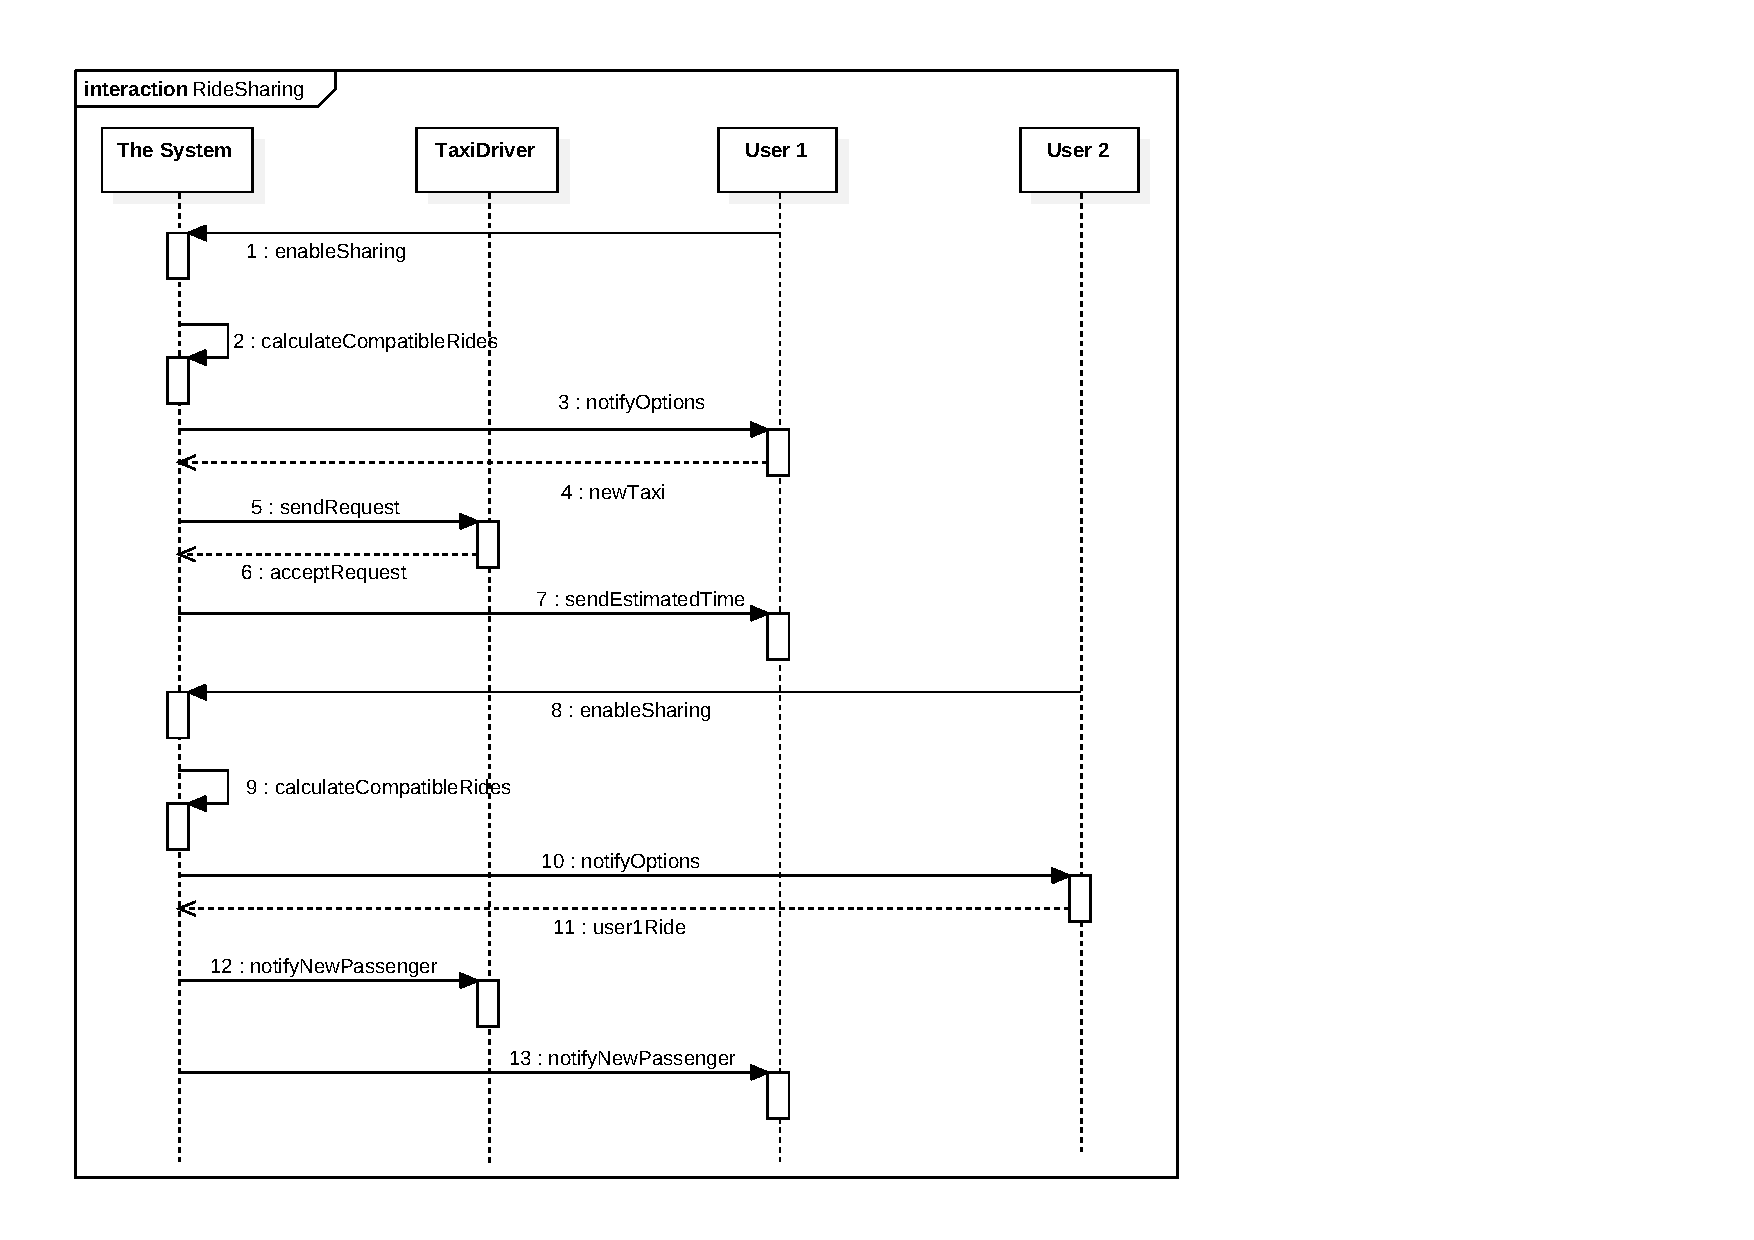
\includegraphics[width=0.9\textwidth]{diagrams/sequence_ride_sharing.pdf}
	\caption{Sequence diagram of a ride sharing with 2 passengers.}
	\label{fig:sequence-sharing}
\end{figure}

\subsubsection{Associated functional requirements}
\begin{enumerate}
	\item The system has to know the position of the new passenger in order to provide feasible sharing solutions.
	It has to compute the estimated walking time to reach the meeting location and compare it with the estimated taxi arrival time.
	\item The passenger can enable the sharing function both in the mobile app and in the web interface.
	\item The passenger can choose between possible sharing solutions or a new taxi.
	\item The system has to communicate to the taxi driver the presence of a new passenger.
<<<<<<< Updated upstream
	\item The system must be able to know if the taxi driver has already picked up the travelers or not.
	\item The system must be able to know how many travelers are currently in the taxi and what is the next scheduled destination.
	\item The total number of travelers must not exceed the number of seats available in each taxi.
	\item The taxi driver has to insert the number of passengers who have been picked up.
	\item After the user chooses to enable the sharing mode, the system has to list all the locations and times of the feasible shared rides.
	\item The system splits the ride costs among the passengers, considering the number of travelers linked to a passenger.
=======
	\item The system must be able to know if the taxi driver has already picked up the travellers or not.
	\item The system must be able to know how many travellers are in the taxi and what is the next scheduled destination.
	\item The total number of travellers must not exceed the number of seats available in each taxi.
	\item The taxi driver can insert the number of passengers who have been picked up.
	\item After the user chooses to enable the sharing mode, the system has to specify, for every sharing ride, the location and the time.
	\item The system splits the ride costs among the passengers, considering the number of travellers linked to a passenger.
>>>>>>> Stashed changes
	\begin{enumerate}
		\item The fee for each passenger is reported by the system as a percentage, because the system knows nothing about the taxi fees in each city.
		\item The fee for each traveller is computed as follows: for each traveller the system computes the total distance travelled, from the starting point to his or her destination. Then the system divides the distance travelled by each traveller by the sum of all the distances.
		\item The system reports to each passenger the fee, as a percentage, summing the fees of all the travellers he/she brought with him/her.
	\end{enumerate}
	\item The system reports all the percentages of the fees to the taxi driver and to all the passengers.
\end{enumerate}
